\documentclass[a4paper,12pt,oneside,openright,extrafontsizes,openbib]{memoir}
%Define o tamanho da fonte para os título das seções primárias (Large)
\chapterstyle{section}
\renewcommand*{\chapnumfont}{\normalfont\Large\bfseries}
\renewcommand*{\chaptitlefont}{\normalfont\Large\bfseries}
%Algarismos arábicos nas páginas
\pagenumbering{arabic}
%Estilo de página
\pagestyle{simple}
%Define a PARTE (da classe Memoir) sem numeração de páginas.
\aliaspagestyle{part}{empty}
%Define secionamento numerado até a seção quaternária.
\settocdepth{subsubsection}
\setsecnumdepth{subsubsection}
%Config. das notas de rodapé.
\setlength{\footmarkwidth}{0em}
%Espaçamento de 1pt entre os parágrafos.
\setlength{\parskip}{1\baselineskip}
%Define a indentação padrão do parágrafos.
\setlength{\parindent}{1.25cm}
%Define o espaçamento entre linhas (exceto para citações longas).
\OnehalfSpacing
%========================================================
%PACOTES ESPECÍFICOS POR ÁREA DE ESTUDO/PESQUISA
%INÍCIO COMPUTAÇÃO
%Caixas de texto para inserção de códigos. Suporta diferentes linguagens.
\usepackage{codebox}
%Replicar comandos e saídas de um shell.
\usepackage{shdoc}
\shautoformat{true}
%Destacar sintaxe de código em caixa de texto simples.
\usepackage{pygmentex}
%FIM COMPUTAÇÃO
%========================================================
%Geometria do tipo de papel (A4).
\usepackage[a4paper,%
		left=3cm,%
		right=2cm,% 
		top=3cm,% 
		bottom=2cm]{geometry}
%Medir margens do pacote Geometry.
\usepackage{calc}
%Fonte 10pt para legendas de figuras e tabelas
\usepackage[font=footnotesize]{caption}
%Gerar Lorem Ipsum.
\usepackage{lipsum}
%Idiomas (o último é o principal do documento).
\usepackage[spanish,english,brazil]{babel}
%Inserir acentos .
\usepackage[utf8]{inputenc}
%Tipo de fonte usada na compilação para incluir caracteres com acentos (Ö, é, à).
\usepackage[T1]{fontenc}
%Microtipografia conforme a língua utilizada.
\usepackage[babel=true]{microtype}
%Controle e personalização de listas
\usepackage{enumitem}
\setlist{nosep}
%Hiperlinks internos e externos.
%Esconder caixa vermelha das hiperligações no documento.
%Ativar links clicáveis no pdf, com cor azul.
\usepackage[breaklinks,%
		hidelinks,%
		colorlinks=true,%
		allcolors=blue]{hyperref}
%Digitar URL completas e clicáveis. 
%Caso queira links com a cor igual ao texto (preto), mudar acima para 'colorlinks=false'.
\usepackage{xurl}
%Para escrever códigos ou trechos de códigos. Ver ambiente CODEX.
\usepackage{verbatim}
%Para escrever versos. Funciona como o verbatim.
\usepackage{alltt}
%inserir imagens.
\usepackage{graphicx}
%Inserir páginas PDF.
\usepackage{pdfpages}
%Criar multicolunas sem o ambiente "tabular".
\usepackage{multicol}
%Caixas de alerta. Útil para livros didáticos ou destaque de algum trecho importante.
\usepackage{alertmessage}
%Cores.
\usepackage{xcolor}
%Diagramas.
\usepackage{smartdiagram}
%Tabelas mais fáceis.
\usepackage{tabularx}
%Mais controle e personalização em tabelas.
\usepackage{booktabs}
%Mudar espaçamento entre linhas.
\usepackage{setspace}
%Indentação de todos os primeiros parágrafos.
\usepackage{indentfirst}
%Digitar aspas com \qq e \q.
\usepackage{textcmds}
%Fonte padrão do documento.
\usepackage{times}
%Facilidades para manipualar formatação de FONTES (riscado, espaçamento entre carcateres...).
\usepackage{soul}
%Destaca a primeira letra do parágrafo. Fonte maior e em caixa de texto.
\usepackage{lettrine}
%Símbolos fonéticos.
\usepackage{tipa}
%CAIXAS DE TEXTO
%Caixas de texto "quebráveis entre páginas".
\usepackage{mdframed}
\usepackage{framed}
%TCOLORBOXES
\usepackage{tcolorbox}
\tcbuselibrary{most,listingsutf8}

%Referências e Citações
\usepackage[alf,
            abnt-emphasize=bf,%
            abnt-etal-list=3,%
            abnt-etal-text=emph,%
            abnt-missing-year=sd,%
            abnt-repeated-author-omit=yes,%
            abnt-repeated-title-omit=yes,%
            abnt-thesis-year=final,%
            abnt-doi=link,%
            ]{abntex2cite}

%AMBIENTES PERSONALIZADOS
%Verbatim modificaddo para incluir códigos em listas.
%\newenvironment{mverbt}
%{\verbatim}%
%{\endverbatim}

%Para citações longas.
\newenvironment{citel}
{\SingleSpacing\small\list{}{\rightmargin=0cm \leftmargin=4cm}%
	\item\relax}%
{\endlist}

%Texto da folha de rosto (tipo de trabalho).
\newenvironment{textofolharosto}
{\SingleSpacing\small\list{}{\rightmargin=0cm \leftmargin=7cm}%
	\item\relax}%
{\endlist}

%Ambiente de caixa: CODEX.
\newtcblisting[auto counter,number within=chapter]{codex}[2][]{%
				arc=0mm,
				listing only,
				colback=black!5!white,
				colframe=black!85!white,
				fonttitle=\bfseries,
				title=Exemplo \thetcbcounter: #1 #2,
				listing options={style=tcblatex,%
								numbersep=1mm,%
								numbers=left,%
								numberstyle=\tiny\color{black}}
}
%Ambiente de caixa: OBSERVAÇÃO
\newtcolorbox{observ}[1][]{%
					arc=0mm,
					listing only,
					colback=black!5!white,
					colframe=red,
					fonttitle=\bfseries,
					title=Observação: #1,
}

%TCOLORBOX com molduras coloridas.
%Ambiente mvermelha
\colorlet{redbx}{red!75!black}
\newtcolorbox{mvermelha}[1]{%
	title={#1},
	empty,
	attach boxed title to top left,
	boxed title style={empty,size=minimal,
		toprule=2pt,top=4pt,
		overlay={\draw[redbx,line width=2pt]
			([yshift=-1pt]frame.north west)--([yshift=-1pt]frame.north east);}},
	coltitle=redbx,
	fonttitle=\Large\bfseries,
	before=\par\medskip\noindent,parbox=false,boxsep=0pt,left=0pt,right=3mm,top=4pt,
	breakable,pad at break*=0mm,vfill before first,
	overlay unbroken={\draw[redbx,line width=1pt]
		([yshift=-1pt]title.north east)--([xshift=-0.5pt,yshift=-1pt]title.north-|frame.east)
		--([xshift=-0.5pt]frame.south east)--(frame.south west); },
	overlay first={\draw[redbx,line width=1pt]
		([yshift=-1pt]title.north east)--([xshift=-0.5pt,yshift=-1pt]title.north-|frame.east)
		--([xshift=-0.5pt]frame.south east); },
	overlay middle={\draw[redbx,line width=1pt] ([xshift=-0.5pt]frame.north east)
		--([xshift=-0.5pt]frame.south east); },
	overlay last={\draw[redbx,line width=1pt] ([xshift=-0.5pt]frame.north east)
		--([xshift=-0.5pt]frame.south east)--(frame.south west);},%
}

%Ambiente mverde
\colorlet{greenbx}{green!75!black}
\newtcolorbox{mverde}[1]{%
	empty,title={#1},attach boxed title to top left,
	boxed title style={empty,size=minimal,toprule=2pt,top=4pt,
		overlay={\draw[greenbx,line width=2pt]
			([yshift=-1pt]frame.north west)--([yshift=-1pt]frame.north east);}},
	coltitle=greenbx,fonttitle=\Large\bfseries,
	before=\par\medskip\noindent,parbox=false,boxsep=0pt,left=0pt,right=3mm,top=4pt,
	breakable,pad at break*=0mm,vfill before first,
	overlay unbroken={\draw[greenbx,line width=1pt]
		([yshift=-1pt]title.north east)--([xshift=-0.5pt,yshift=-1pt]title.north-|frame.east)
		--([xshift=-0.5pt]frame.south east)--(frame.south west); },
	overlay first={\draw[greenbx,line width=1pt]
		([yshift=-1pt]title.north east)--([xshift=-0.5pt,yshift=-1pt]title.north-|frame.east)
		--([xshift=-0.5pt]frame.south east); },
	overlay middle={\draw[greenbx,line width=1pt] ([xshift=-0.5pt]frame.north east)
		--([xshift=-0.5pt]frame.south east); },
	overlay last={\draw[greenbx,line width=1pt] ([xshift=-0.5pt]frame.north east)
		--([xshift=-0.5pt]frame.south east)--(frame.south west);},%
}

%Caixas de textto com MDFRAMED
\newenvironment{bxpreta}
{\begin{mdframed}
		[skipabove=7pt,
		skipbelow=7pt,
		rightline=false,
		leftline=true,
		topline=false,
		bottomline=false,
		backgroundcolor=black!5,
		linecolor=black,
		innerleftmargin=5pt,
		innerrightmargin=5pt,
		innertopmargin=5pt,
		innerbottommargin=5pt,
		leftmargin=0cm,
		rightmargin=0cm,
		linewidth=5pt]}
	{\end{mdframed}}

\newenvironment{bxlaranja}
{\begin{mdframed}
		[skipabove=7pt,
		skipbelow=7pt,
		rightline=false,
		leftline=true,
		topline=false,
		bottomline=false,
		backgroundcolor=black!5,
		linecolor=orange,
		innerleftmargin=5pt,
		innerrightmargin=5pt,
		innertopmargin=5pt,
		innerbottommargin=5pt,
		leftmargin=0cm,
		rightmargin=0cm,
		linewidth=5pt]}
	{\end{mdframed}}

%Caixa Fundo cinza, Borda cinza
\newenvironment{bxcinza}
{\begin{mdframed}
		[skipabove=7pt,
		skipbelow=7pt,
		rightline=false,
		leftline=true,
		topline=false,
		bottomline=false,
		linecolor=gray,
		backgroundcolor=black!5,
		innerleftmargin=5pt,
		innerrightmargin=5pt,
		innertopmargin=5pt,
		leftmargin=0cm,
		rightmargin=0cm,
		linewidth=4pt,
		innerbottommargin=5pt]}
	{\end{mdframed}}

%Caixa Fundo azul, Borda azul
\newenvironment{bxazul}
{\begin{mdframed}
		[skipabove=7pt,
		skipbelow=7pt,
		rightline=false,
		leftline=true,
		topline=false,
		bottomline=false,
		linecolor=blue!40!gray,
		backgroundcolor=black!5,
		innerleftmargin=5pt,
		innerrightmargin=5pt,
		innertopmargin=5pt,
		leftmargin=0cm,
		rightmargin=0cm,
		linewidth=4pt,
		innerbottommargin=5pt]}
	{\end{mdframed}}

%Borda vermelha
\newenvironment{bxvermelha}
{\begin{mdframed}
		[skipabove=7pt,
		skipbelow=7pt,
		rightline=false,
		leftline=true,
		topline=false,
		bottomline=false,
		backgroundcolor=black!5,
		linecolor=red!40!gray,
		innerleftmargin=5pt,
		innerrightmargin=5pt,
		innertopmargin=5pt,
		innerbottommargin=5pt,
		leftmargin=0cm,
		rightmargin=0cm,
		linewidth=5pt]}
	{\end{mdframed}}

\begin{document}
%NÃO ALTERAR O TRECHO ABAIXO. SÃO AS CONFIGS. DOS PRÉ-TEXTUAIS.
    \begin{titlingpage}
	%PREENCHA OS CAMPOS ABAIXO COM AS INFORMAÇÕES DO SEU TRABALHO
%SUBSTITUA OS EXEMPLOS
\author{Leocádio Nestor Gumercindo Filho}
\title{A representação do arco-íris no Reino dos Unicórnios:\\ uma aplicação da variável CORES PRIMÁRIAS}
%Data da defesa. Apenas mês e ano.
\date{Jan. 2050}

%INFORMAÇÕES DA INSTITUIÇÃO E CURSO
\newcommand{\instituicao}{Instituto Federal de Pernambuco}
\newcommand{\campus}{Campus Garanhuns}
\newcommand{\curso}{Análise e desenvolvimento de sistemas}
\newcommand{\titulacao}{Tecnólogo}%Ou bacharel, ou licenciado.
\newcommand{\localdefesa}{Garanhuns - PE}
%Data exata da defesa para a folha de aprovação.
\newcommand{\dataexatadefesa}{01 de jan. \the\year}

%INFORMAÇÕES DO ORIENTADOR/A
\newcommand{\orientador}{Nome Completo do/a Orientador/a}
%Mude o texto da linha abaixo conforme o gênero do orientador/a.
\newcommand{\printorientador}{(Orientador/a)}
%Substitua "Titulação do orientador" por Esp., Me., Ma., Dr. ou Drª
\newcommand{\titorientador}{Dr.}
%Altere a linha abaixo caso seu orientador não seja do IFPE Garanhuns
\newcommand{\localorientador}{Instituto Federal de Pernambuco Campus Garanhuns}

%INFORMAÇÕES DOS AVALIADORES
%Avaliador/a 1
\newcommand{\avaliadorum}{Nome Completo do/a Avaliador/a 1}
\newcommand{\titavaliadorum}{Drª}% Esp., Me., Ma., Dr. ou Drª
\newcommand{\localavalum}{Universidade Floresta Mágica}% UFRPE, UFPE, UFMG etc por extenso
%Avaliador/a 2
\newcommand{\avaliadordois}{Nome Completo do/a Avaliador/a 1}
\newcommand{\titavaliadordois}{Me.}% Esp., Me., Ma., Dr. ou Drª
\newcommand{\localavaldois}{Instituto Bosque das Flores}% UFRPE, UFPE, UFMG etc por extenso

%FORMATAÇÃO DO ELEMENTOS PRÉ-TEXTUAIS - NÃO ALTERAR
%Capa
\begin{center}
%CAPA
%CASO NÃO DESEJE O LOGO DA INSTITUIÇÃO, EXCLUIR LINHA ABAIXO.

\includegraphics[scale=.10]{./img/logo-ifpe.png}\\
\textbf{\textsc{\instituicao}}\\
%Caso sua instituição não tenha CAMPUS, remova o comando \campus.
\textbf{\textsc{\campus}}\\
\textbf{\textsc{\curso}}


\vspace*{5cm}
\textbf{\thetitle}\\
\textbf{\theauthor}

\vspace*{\fill}
\localdefesa\\
\thedate
\end{center}

%FOLHA DE ROSTO + TIPO DE TRABALHO
\frontmatter{
\newpage
\thispagestyle{empty}
\begin{center}
    \textbf{\theauthor}
	
    \vspace*{5cm}
    \textbf{\thetitle}
\end{center}
%Caso sua instituição não tenha CAMPUS, remova o comando \campus.
%ATENÇÃO À PREPOSIÇÃO "AO/À"
\vspace*{2cm}
    \begin{textofolharosto}
    Trabalho de conclusão de curso apresentado ao/à \instituicao\ \campus\ como requisito parcial para obtenção do título de \titulacao\ em \curso.\\
    \ \\
    \textbf{Orientador:} \orientador
    \end{textofolharosto}

\begin{center}
\vspace*{\fill}
    \localdefesa\\
    \thedate
\end{center}

%FICHA CATALOGRÁFICA.
%Após a confecção da ficha catalográfica pela biblioteca de sua instituição --
%aqui, a biblioteca do IFPE Campus Garanhuns --
%imprima o arquivo (provavelmente em .docx) para pdf e salve-o
%na pasta pretxt do projeto com o nome "fichacatalografica.pdf".
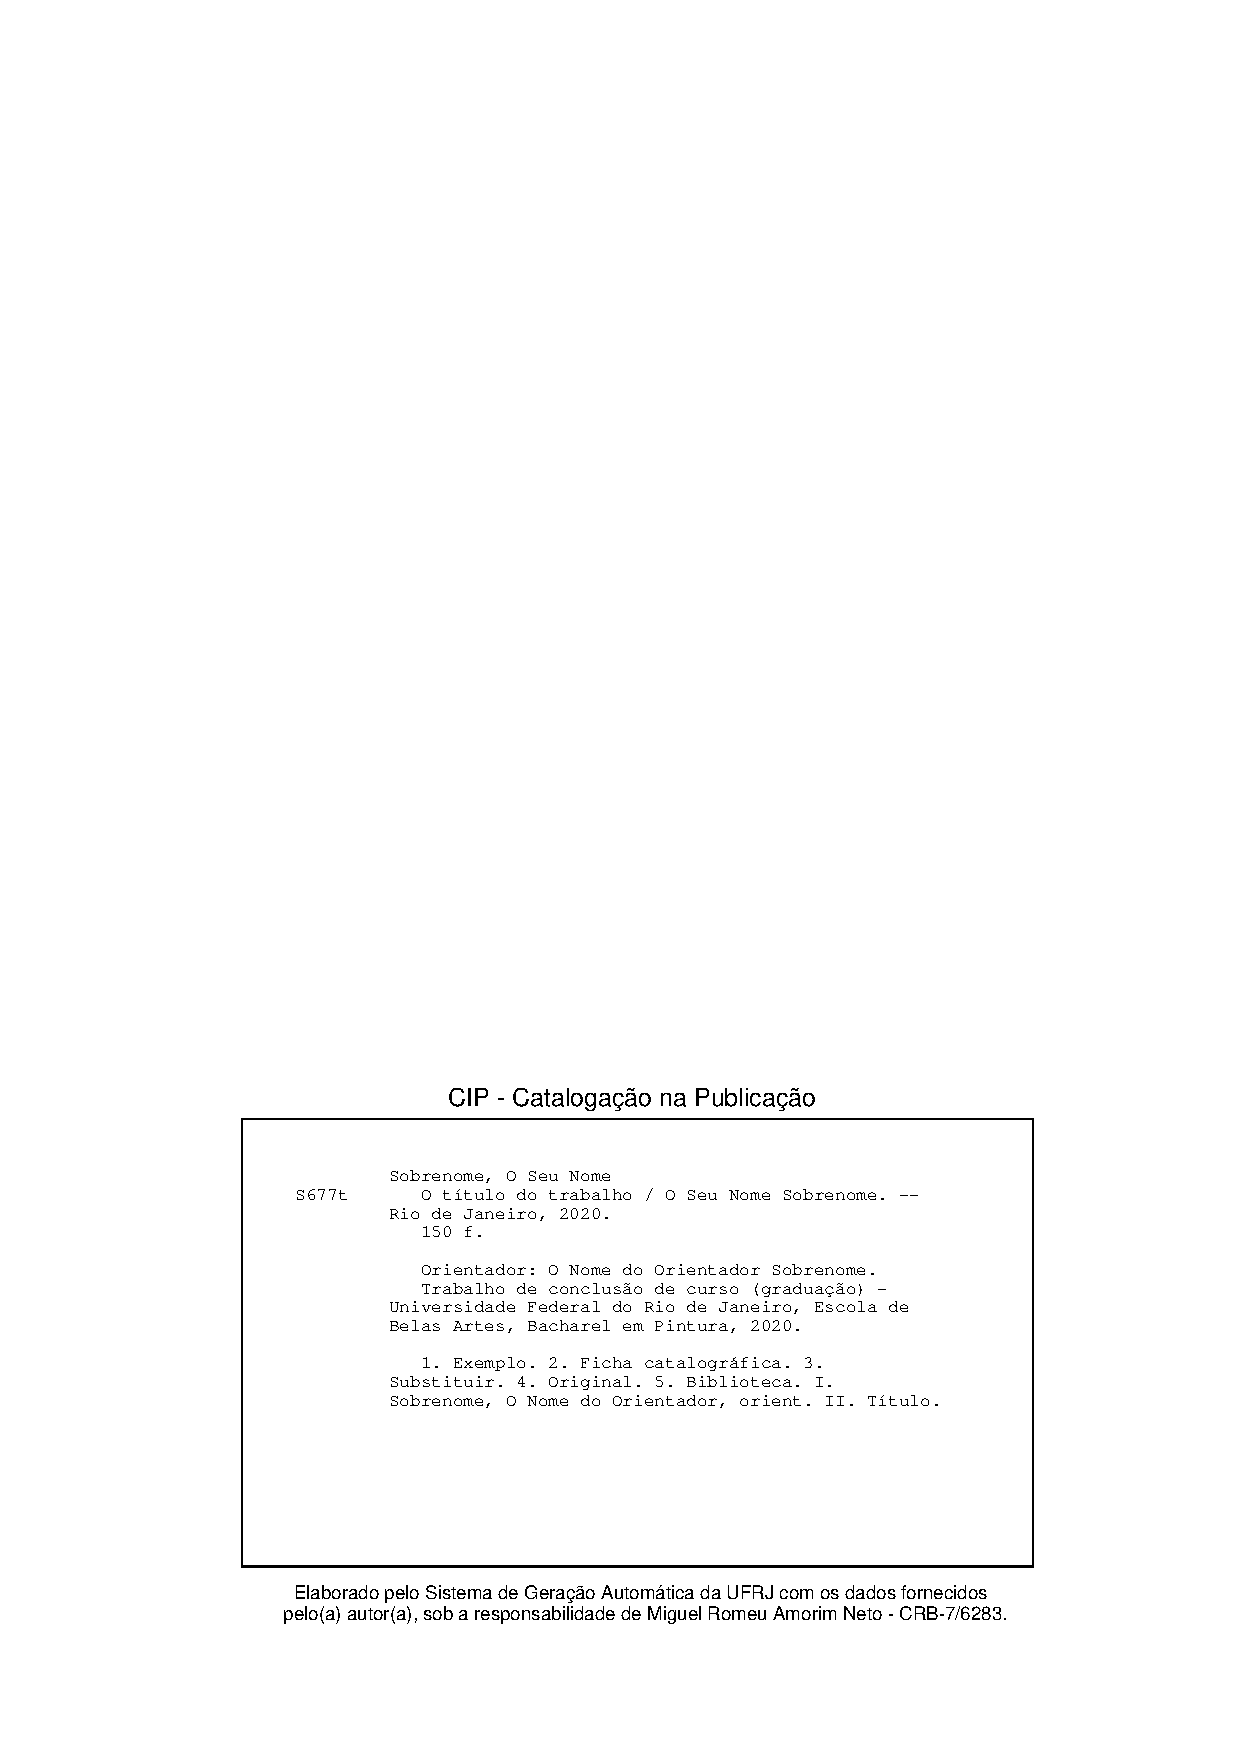
\includepdf{fichacatalografica.pdf}

%FOLHA DE APROVAÇÃO
\newpage
\thispagestyle{empty}
\begin{center}
    \textbf{\textsc{\theauthor}}
	
    \textbf{\textsc{\thetitle}}
%ATENÇÃO AO USO DA PREPOSIÇÃO (DO/DA) ANTES DO COMANDO \instituicao	
\vspace*{2cm}
    \begin{textofolharosto}
        Este Trabalho de Conclusão de Curso foi julgado adequado para obtenção do Título de \titulacao\ e aprovado em sua forma final pelo Curso de \curso\ da \instituicao\ \campus.\\
        \ \\
        \ \\
        \localdefesa\ \-- \dataexatadefesa
        \end{textofolharosto}
	
        \vspace*{2cm}
        \line(1,0){10cm}\\
        \textbf{\titorientador\ \orientador\ \printorientador}\\
        \localorientador\\
        	
        \vspace*{2cm}
        \line(1,0){10cm}\\
        \textbf{\titavaliadorum\ \avaliadorum}\\
        \localavalum\\
        	
        \vspace*{2cm}
        \line(1,0){10cm}\\
        \textbf{\titavaliadordois\ \avaliadordois}\\
        \localavaldois
    \end{center}

%EPÍGRAFE
\newpage
\thispagestyle{empty}
\vspace*{\fill}
\epigraph{\textit{Uma frase importante relacionada ao trabalho.}}{\textsc{Quem disse a frase.}}

%DEDICATÓRIA
\newpage
\thispagestyle{empty}
\vspace*{15cm}
\begin{flushright}
    \SingleSpacing\textit{Dedico este trabalho ao ilustríssimo Professor Dr. André Padilha por ter me fornecido esse modelo de trabalho em \LaTeX\ e facilitar minha jornada na escrita acadêmica.}
\end{flushright}

%AGRADECIMENTOS
\newpage
\pagestyle{empty}
\begin{center}
	\textbf{\textsc{Agradecimentos}}
\end{center}
% Digite os agradecimentos a partir da linha abaixo 
% e SEMPRE após o comando no indent, após o primeiro
% afradecimento. EXEMPLO:
Agradeço incomensuravelmente ao ilustríssimo Professor Dr. André Padilha por ter me fornecido esse modelo de trabalho em \LaTeX\ e facilitar minha jornada na escrita acadêmica.

\noindent Abaixo, o resto dos agradecimentos...

\noindent Ao papai.

\noindent À mamãe.

\noindent Ao meu papagaio José Eustáquio. 

\noindent Ao \textit{Lorem ipsum}, abaixo.

\noindent  \lipsum[10]

%RESUMO e ABSTRACT
\newpage
\pagestyle{empty}
\begin{center}
    \textbf{\textsc{Resumo}}
\end{center}
\SingleSpacing\noindent
    O resumo de um trabalho acadêmico é normatizado pela ABNT 6028:2018. Deve ser escrito em 3ª pessoa, ter entre 150 a 500 palavras e apresentar: \textit{finalidades (objetivos), metodologia, referencial teórico, resultados e conclusões}. Deve ser escrito em bloco único, com frases concisas. Para trabalhos de graduação, a prática mais comum é ter até 300 palavras.

\vspace*{0.5cm}
\noindent\textbf{Palavras-chave:} Palavra 1; Palavra 2; Palavra 3. (Até cinco, separadas por \q{ ; } (ponto e vírgula).

%ABSTRACT
\newpage
\pagestyle{empty}
\begin{center}
    \textbf{\textsc{Abstract}}
\end{center}
\SingleSpacing\noindent
    Write your abstract here. Follow the same rules as indicated previously. Avoid using any automatic translation tool as \textit{Google Translator} except if you know what you are doing.

\vspace*{0.5cm}
\noindent\textbf{Keywords:} Word 1; Word 2; Word 3.
}
\newpage
\tableofcontents*
\thispagestyle{empty}
\newpage\listoffigures*
\thispagestyle{empty}
\newpage\listoftables*
\thispagestyle{empty}
    \end{titlingpage}
%INÍCIO DOS ELEMENTOS TEXTUAIS (CAPS./SEÇÕES)
\mainmatter{
\chapter*{Apresentação}\label{ch:apres}
\addcontentsline{toc}{chapter}{Apresentação}
Este modelo de documento foi elaborado para atender às necessidades dos estudantes dos cursos de graduação do IFPE Campus Garanhuns.

Quaisquer modificações que eventualmente venham a ser feita devem ocorrer no arquivo \textbf{definicoes.tex} e obedecer à estrutura do projeto. Veja o README.md no Github para explicações adicionais.

%Nome do seu capítulo/seção 1. Use a ref. cruzada como em \label
\chapter{Pacotes e ambiente incluídos}\label{ch:01}
Para detalhes sobre os pacotes incluídos nesse modelo, veja o arquivo \textbf{definicoes.tex} para informações básicas ou acesse os \textit{links} disponíveis ao longo do documento para ler a documentação. 

Os exemplos de uso, incluindo o código \LaTeX, de cada um deles estão na seção Apêndices.

\section{Lettrine}\label{sec:Lettrine}

\lettrine[findent=2pt]{\fbox{\textbf{V}}}{eja essa frase de abertura...} \lipsum[1]

\textsc{Pacote:} lettrine

Acesso: \url{https://www.ctan.org/pkg/lettrine}

\section{Verbatim}\label{sec:Verbatim}

\textsc{Pacote:} verbatim

Acesso: \url{https://www.ctan.org/pkg/verbatim}

\section{Inserir páginas em .pdf}\label{sec:pdfpages}

\textsc{Pacote:} pdfpages

\url{https://www.ctan.org/pkg/pdfpages}

\section{Texto em várias colunas}\label{sec:multicol}

\textsc{Pacote:} multicol

\url{https://www.ctan.org/pkg/multicol}

Outra possibilidade de inserção de texto em mais de uma coluna em uma página é através do uso de tabelas ou do ambiente \verb|minipage|. 

Para esse último, o código básico é:

\begin{codex}{Ambiente minipage básico}
    \begin{minipage}{4cm}
       Os {4cm} indicados acima apontam para a largura desejada da "minipage". 
    \end{minipage}
\end{codex}

Veja \url{https://www.alessandroduarte.com.br/?page_id=602} para um tutorial em português.

\section{Diagramas}\label{sec:smartdiagram{}

\textsc{Pacote:} smartdiagram

\url{https://www.ctan.org/pkg/smartdiagram}

\section{Aspas e outros símbolos tipográficos}\label{sec:textcmds}

\textsc{Pacote:} textcmds

\url{https://ctan.math.illinois.edu/macros/latex/contrib/amsrefs/textcmds.pdf}

Esse pacote foi incluído porque em modo \textit{offline} o \LaTeX habitualmente não reconhece os espaços necessários entre as aspas. O Overleaf já o faz nativamente (embora eu tenha observado erros nas aspas simples...).

\section{Hiperlinks com quebra de endereço por linha}\label{sec:xurl}

\textsc{Pacote:} xurl

\url{https://www.ctan.org/pkg/xurl}

\section{Tabelas}\label{sec:tabularx}

\textsc{Pacote:} tabularx

\url{https://www.ctan.org/pkg/tabularx}

\section{Imagens}\label{sec:graphicx}

\textsc{Pacote:} graphicx

\url{https://www.ctan.org/pkg/graphicx}

\section{Inserção de códigos de programação}\label{sec:codes}

\textsc{Importante:} Somente consegui reproduzir no Overleaf o pacote \verb|codebox|. Os pacotes \verb|shdoc| e \verb|pygmentex| não compilaram adequadamente, resultando em erros. Sugiro que tentem no modo \textit{offline} (\LaTeX\ instalado no computador).

\subsection{codebox}\label{subsec:codebox}
\textsc{Pacote:} codebox

\url{https://www.ctan.org/pkg/codebox}

\subsection{shdoc}\label{subsec:shdoc}
\textsc{Pacote:} shdoc

\url{https://www.ctan.org/pkg/shdoc}

\subsection{pygmentex}\label{subsec:pygmentex}
\textsc{Pacote:} pygmentex

\url{https://www.ctan.org/pkg/pygmentex}

\section{Ambientes \LaTeX\ personalizados}\label{sec:personal}

\subsection{codex}\label{subsec:codex}

\subsection{observ}\label{subsec:observ}

\subsection{citel}\label{subsec:citel}

\subsection{Caixas de Texto}\label{subsec:caixatextos}

Há diversos ambientes possíveis para criar caixas de texto neste modelo. São eles:

\begin{enumerate}
    \item codex
    \item observ
    \item mverde
    \item mvermelha
    \item bxpreta
    \item bxlaranja
    \item bxcinza
    \item bxazul
    \item bxvermelha
    \item \textbf{alertmessage\footnote{Exceção aos listados acima. Trata-se de um comando, não de um ambiente.}}
\end{enumerate}

\textsc{Pacotes:}
\begin{enumerate}
    \item tcolorbox
    \begin{itemize}
        \item Acesso: \url{https://www.ctan.org/pkg/tcolorbox}
    \end{itemize}
    \item framed
    \begin{itemize}
        \item Acesso: \url{https://www.ctan.org/pkg/framed}
    \end{itemize}
    \item mdframed
    \begin{itemize}
        \item Acesso: \url{https://www.ctan.org/pkg/mdframed}
    \end{itemize}
    \item alertmessage
    \begin{itemize}
        \item Acesso: \url{https://www.ctan.org/pkg/alertmessage}
    \end{itemize}
\end{enumerate}

\chapter{Estrutura do projeto}

Esse modelo contém seis arquivos e uma pasta que devem ser enviados para o Overleaf após a criação da conta gratuita na plataforma.

No caso de uso \textit{offline} do \LaTeX, descompacte o .zip baixado do GitHub para uma pasta e siga as mesmas orientações.

\section{definicoes.tex}

Contém todas as definições do modelo conforme a ABNT 14721:2011 além de todos os pacotes e ambientes utilizados. Ver os \textbf{Apêndices} para uma explicação dos comandos e ambientes.

\section{pretextuais.tex}

Estão todas as informações necessárias ao projeto, tais como:

\begin{itemize}
    \item Capa
    \item Folha de rosto
    \item Ficha catalográfica (ver explicação abaixo)
    \item Folha de aprovação
    \item Epígrafe
    \item Dedicatória
    \item Agradecimentos
    \item Resumo e Abstract
\end{itemize}

É nesse arquivo que as informações do estudante, título do trabalho, orientador, avaliadores, etc estão incluídas. \textsc{LEIA ESSE ARQUIVO COM ATENÇÃO.}

\section{fichacatalografica.pdf}

Normalmente, a ficha catalográfica é feita por um/uma bibliotecário/a e entregue em formato .doc, .docx ou .odt. 

Após a elaboração pelo/a profissional responsável, imprima/converta esse arquivo para .pdf e substitua o arquivo \verb|fichacatalografica.pdf| que já vem no projeto.

\section{textuais.tex}

É o arquivo onde se digitam as seções (capítulos) do seu trabalho. Atentar para a primeira seção (Apresentação). A ABNT 14724:2011 não informa que esta deva ser não-numerada. Por prática, o projeto apresenta essa seção não numerada e incluída já no \textbf{Sumário}.

\section{referencias.bib}

Contém exemplos em branco para auxiliar o preenchimento das referências bem como exemplos já preenchidos para servirem de modelos.

Alguns exemplos de citação vazia seguem abaixo.

\cite{Smurf1980} - Citação direta de artigo, sem fazer parte do texto.

\cite[p. 654]{Vingadores2015} - citação direta de livro com página, sem fazer parte do texto.

\citeonline{Flintstones1900} - citação direta de um livro com Organizador (Org.), sem fazer parte do texto.

\citeonline[p. 89]{Flintstones1900} - a mesma citação acima, com indicação da página.

\cite{Vingadores2016} - citação direta de uma dissertação de mestrado, sem fazer parte do texto. (Ver próxima citação e referência)

\cite{Thor2017} - citação direta de uma tese de doutorado, sem fazer parte do texto e com mesmo autor da citação acima. Observar as \textbf{Referências}.

\section{postextuais.tex}

Contém os Anexos e os Apêndices. Estes são elementos opcionais e, neste modelo, na parte específica dos Apêndices, trazem os exemplos de códigos, pacotes e/ou ambientes utilizados.

\section{pasta img}

Contém as imagens utilizadas no projeto. Use o formato .png e .jpg para não precisar instalar pacotes extras ou \qq{quebrar muito a cabeça} com conversões entre formatos.

\chapter{Referências e Citações}\label{ch:refs-cit}

Para a utilização correta do pacote \verb|abntex2cite| nesse projeto, é essencial a leitura dos seguintes materiais disponíveis em \url{https://www.ctan.org/pkg/abntex2}, em especial:

\begin{itemize}
    \item \url{https://linorg.usp.br/CTAN/macros/latex/contrib/abntex2/doc/abntex2cite.pdf}
    \item \url{https://linorg.usp.br/CTAN/macros/latex/contrib/abntex2/doc/abntex2cite-alf.pdf}
\end{itemize}

Ambos os pacotes contém exemplos de uso e, também, a acentuação necessária para cada entrada bibliográfica que deve ser inserida no arquivo \verb|referencias.bib|.
\cite{abnt}
%===============================
%FIM DOS ELEMENTOS TEXTUAIS (CAPS./SEÇÕES)
%Não apagar a chave a seguir.
}






%INÍCIO DOS ELEMENTOS PÓS TEXTUAIS (REFERÊNCIAS, ANEXOS, APÊNDICES)
%Início das Referências
\backmatter{
\renewcommand{\bibname}{Referências}
\bibintoc
\bibliographystyle{abntex2-alf}
\bibliography{referencias.bib}
%Fim das Referências
%Se o trabalho não tiver apêndices ou anexos
%excluir ou comentar a linha abaixo.
%ANEXOS
\thispagestyle{empty}
\part*{Anexos} % Se quiser uma página indicativa de ANEXOS antes dos anexos.
\addcontentsline{toc}{part}{Anexos}
%Conforme a norma, os anexos devem se organizar em ordem alfabética: A, B, C, D...
\chapter*{Anexo A -- Um anexo}
\addcontentsline{toc}{chapter}{Anexo A -- Um anexo}


%APÊNDICES
\thispagestyle{empty}
\part*{Apêndices} % se quiser uma página indicativa de APÊNDICES antes dos apêndices
\addcontentsline{toc}{part}{Apêndices}
%Conforme a norma, os apêndices devem se organizar em ordem alfabética: A, B, C, D...
\chapter*{Apêndice A -- lettrine}
\addcontentsline{toc}{chapter}{Apêndice A -- lettrine}

\noindent\textsc{O que faz?}

Desenha uma caixa de texto ao redor da primeira letra da primeira palavra do parágrafo. É um recurso de estilo, apenas.

\lettrine[findent=2pt]{\fbox{\textbf{V}}}{eja essa frase de abertura...} \lipsum[1]

\chapter*{Apêndice B -- verbatim}
\addcontentsline{toc}{chapter}{Apêndice A -- verbatim}

\noindent\textsc{O que faz?}

Digita qualquer coisa fora da formatação do texto, utilizando fonte monoespaçada e conforme os espaçamentos desejados. Útil para pequenos trechos de código.

\begin{codex}{Códigos verbatim}
\verb|comando 1|
    \verb*|comando 2]
        \begin{verbatim}
            qualquer outro texto
        \end{verbatim}
\begin{mverbt}
ambiente personalizado
\item um item de lista
\end{mverbt}
\end{codex}
\begin{multicols}{2}
\setlength{\columnseprule}{0.2pt}
O comando da linha 1, gera o seguinte: \verb|comando 1|.

O comando da linha 2, gera o seguinte: \verb*|comando 2].

Os comandos das linhas 3, 4 e 5 geram o seguinte:
\begin{verbatim}
   qualquer outro texto
\end{verbatim}

Os comandos das linhas 6, 7, 8 e 9 geram o seguinte:
        \begin{mverbt}
        ambiente personalizado
        \item um item de lista
        \end{mverbt}
\end{multicols}
\textbf{Observação:} Notar o alinhamento dos dois últimos ambientes. A tabulação na digitação -- \textit{em verbatim} -- importa para o \LaTeX.


\chapter*{Apêndice C -- pdfpages}
\addcontentsline{toc}{chapter}{Apêndice C -- pdfpages}

\noindent\textsc{O que faz?}

Insere uma ou várias páginas .pdf no arquivo gerado pelo \LaTeX. A numeração é feita de modo automático.

Veja a numeração desta página, note a figura inserida do Tex the Lion e a numeração do \textbf{Apêndice D}. 

Observar o código:
\ \\
\begin{codex}{Inserção de página pdf - Tex the Lion}
    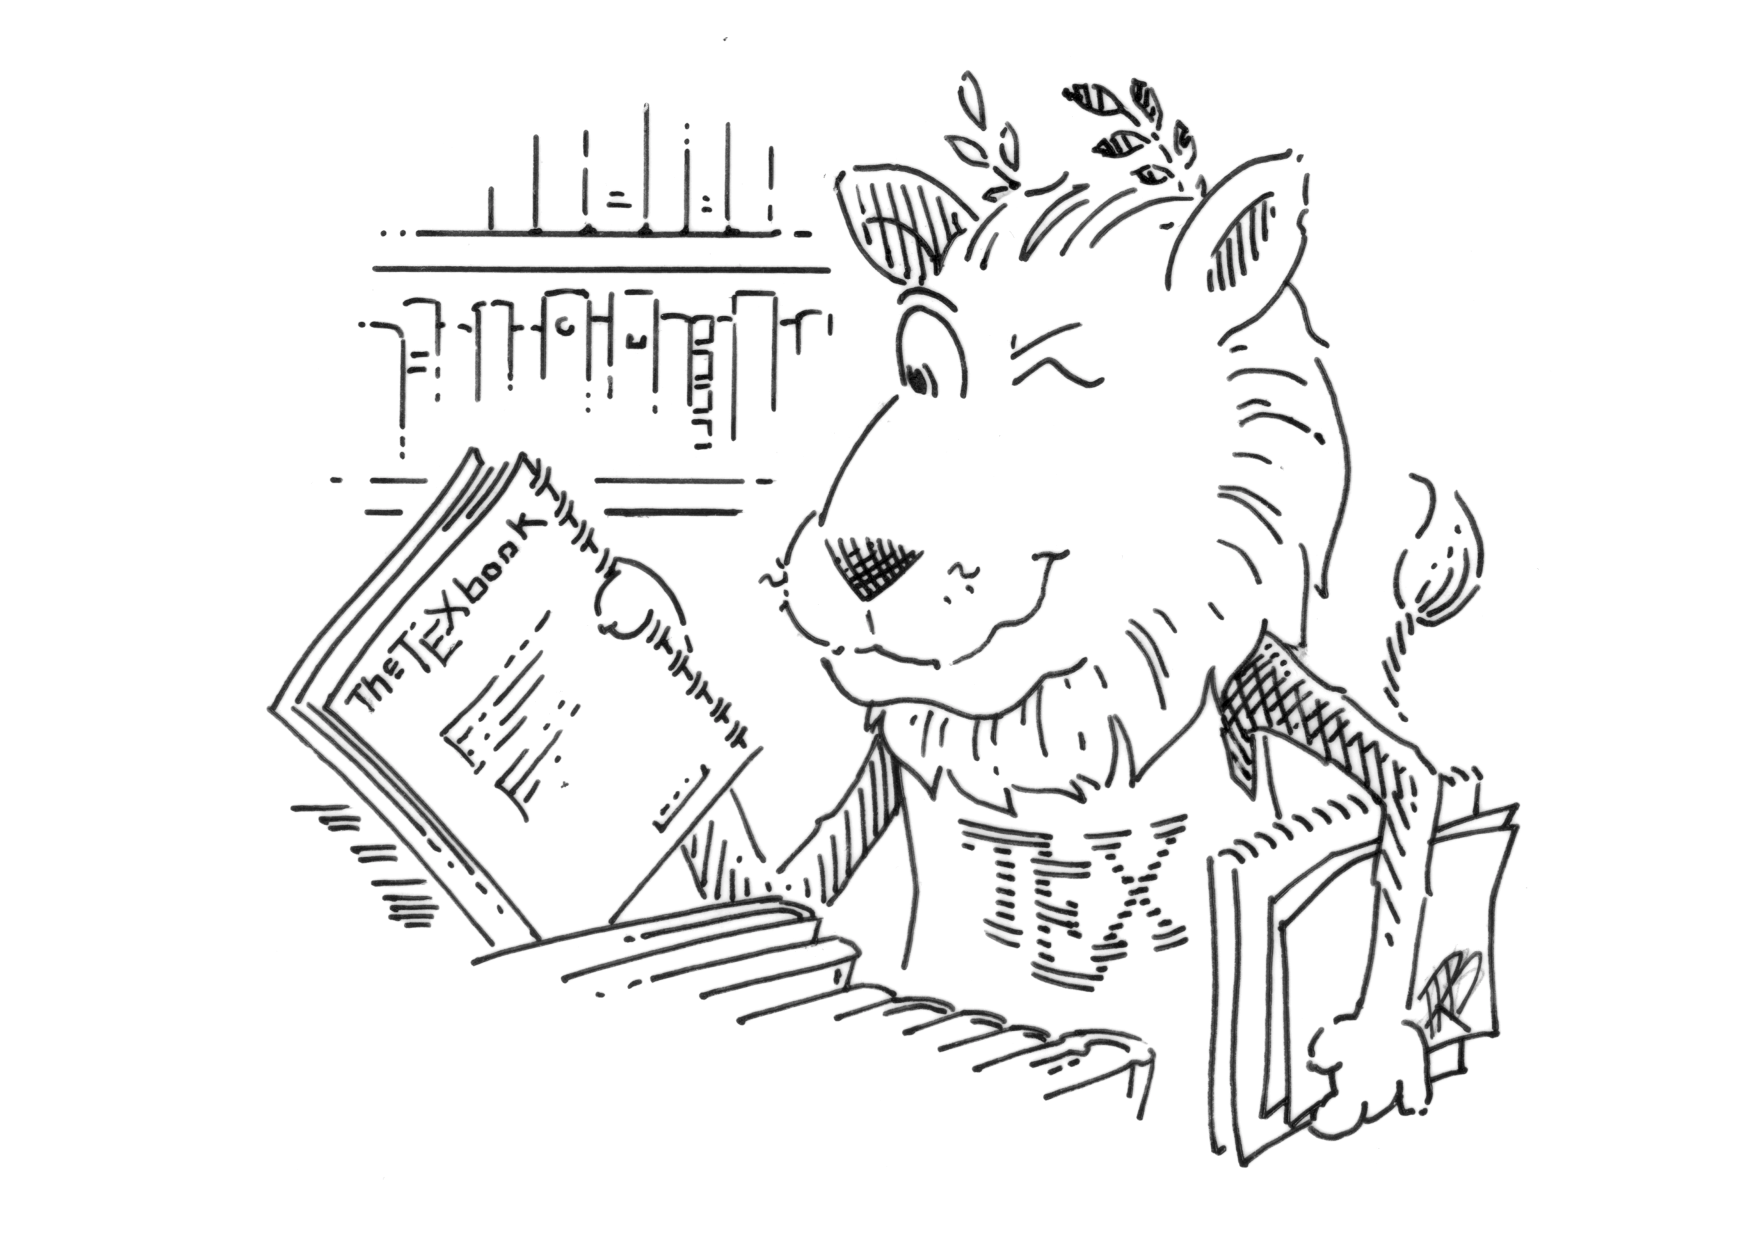
\includepdf[noautoscale=false]{img/tex-lion.pdf}
\end{codex}

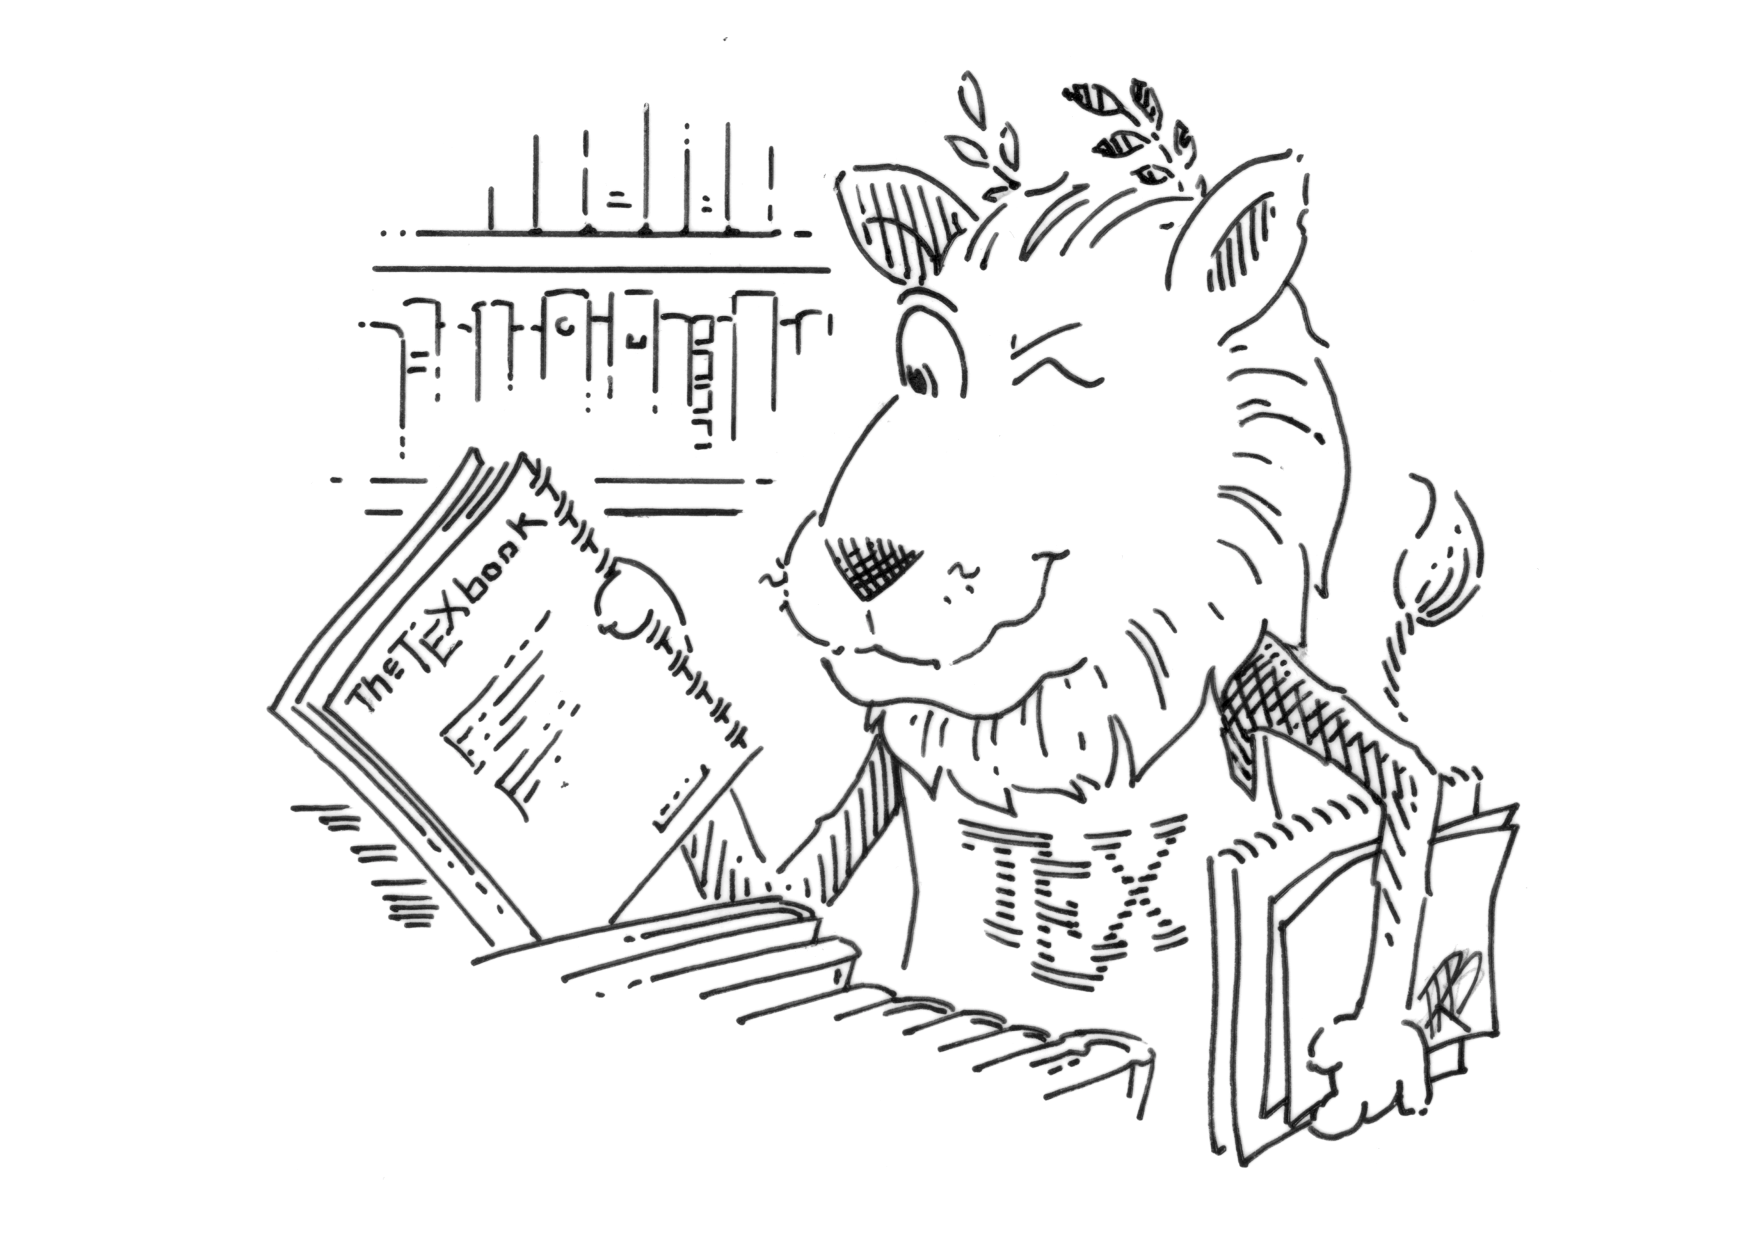
\includepdf[noautoscale=false]{img/tex-lion.pdf}

\chapter*{Apêndice D -- multicol}
\addcontentsline{toc}{chapter}{Apêndice D -- multicol}

\noindent\textsc{O que faz?}

Divide o texto em -- \textit{no máximo} -- 10 colunas. No \textbf{Apêndice C}, tem-se alguns exemplos com o ambiente verbatim.

Observar:

\begin{codex}{Multicolunas com valor 3 e Lorem Ipsum}
    \begin{multicols}{3}
        \lipsum[2]
    \end{multicols}
\end{codex}

\begin{multicols}{3}
        \lipsum[2]
    \end{multicols}

\begin{codex}{Multicolunas com valor 5 e Lorem Ipsum}
    \begin{multicols}{5}
        \lipsum[2]
    \end{multicols}
\end{codex}

\begin{multicols}{5}
        \lipsum[2]
   \end{multicols}

Também é possível incluir uma linha separadora entre as colunas. Ver a seguir.

\begin{codex}{Multicolunas com valor 3 e Lorem Ipsum + Linha}
    \begin{multicols}{3}
    \setlength{\columnseprule}{0.2pt}
    \lipsum[2]
    \end{multicols}
\end{codex}

 \begin{multicols}{3}
    \setlength{\columnseprule}{0.2pt}
    \lipsum[2]
 \end{multicols}

\chapter*{Apêndice E -- smartdiagram}
\addcontentsline{toc}{chapter}{Apêndice E -- smartdiagram}

\noindent\textsc{O que faz?}

Cria diagramas coloridos, em escala de cinza, branco e preto, em formatos diversos a partir de uma lista de itens simples.

\begin{codex}{circular diagram}
\begin{center}
\smartdiagram[circular diagram]{\LaTeX,Digitar,Compilar,Produzir PDF}
\end{center}	
\end{codex}

\begin{center}
	\smartdiagram[circular diagram]{\LaTeX,Digitar,Compilar,Produzir PDF}
\end{center}

\chapter*{Apêndice F -- textcmds}
\addcontentsline{toc}{chapter}{Apêndice F -- textcmds}

\noindent\textsc{O que faz?}
Permite incluir aspas duplas e simples, e outros símbolos tipográficos, com menos esforço na digitação.

Por padrão, o \LaTeX\ produz aspas das seguintes formas:
\begin{enumerate}
	\item SHIFT + acento grave 2x + SHIFT + acento grave 2x + palavra ou expressão entre aspas + aspas simples 2x.
            \begin{itemize}
                \item 'um texto qualquer' entre aspas simples
            \end{itemize}
	\item SHIFT + sinal de acento grave + palavra ou expressão + aspas simples.
            \begin{itemize}
                \item "um texto qualquer" entre aspas duplas
            \end{itemize}
\end{enumerate}

No primeiro exemplo, o 1º sinal das aspas simples não está correto, pois deveria estar voltado para direita.

No segundo exemplo, quando compilado fora do Overleaf, não acrescenta o espaço entre as últimas aspas duplas e a próxima palavra.

Para resolver isso e utilizar \textit{on-line} e \textit{offline} ambas as aspas, use os comandos:

\begin{codex}{Aspas com o pacote textcmds}
Estas são \qq{aspas duplas}.
Estas são \q{aspas simples}.
Estas são \qq{aspas duplas com \q{aspas simples} ao mesmo tempo}
\end{codex}
 Produzirão, respectivamente: Estas são \qq{aspas duplas}; Estas são \q{aspas simples} e Estas são \qq{aspas duplas com \q{aspas simples} ao mesmo tempo}.


\chapter*{Apêndice G -- xurl}
\addcontentsline{toc}{chapter}{Apêndice G -- xurl}

\noindent\textsc{O que faz?}
Permite a quebra de \textit{urls} mesmo quando existem caracteres como \&, \_, \#.

Observe que  caixa de texto, por ser -- também -- um ambiente verbatim, não \qq{quebrará} a url, porém quando digitado em ambiente não verbatim, o endereço é ajustado automaticamente conforme as margens.

\begin{codex}{Exemplo de url longa}
  \url{https://tex.stackexchange.com/questions/341205/what-is-the-difference-between-tabular-tabular-and-tabularx-environments}
\end{codex}
\ \\
Endereço URL ajustado a seguir:

\url{https://tex.stackexchange.com/questions/341205/what-is-the-difference-between-tabular-tabular-and-tabularx-environments}

\chapter*{Apêndice H -- tabularx e booktabs}
\addcontentsline{toc}{chapter}{Apêndice H -- tabularx e booktabs}

\noindent\textsc{O que faz?}

Ambos permitem maior controle de personalização nas tabelas. Reproduzo somente uma simples tabela para fins de estudo do código.

\begin{codex}{Tabela com legenda e referência cruzada}
\begin{table}[h!]
    \begin{center}
	\begin{tabularx}{0.8\textwidth} { 
	| >{\centering\arraybackslash}X 
	| >{\centering\arraybackslash}X 
	| >{\centering\arraybackslash}X | }
	\hline
	item 1 & item 2 & item 3 \\
	\hline
	item 4  & item 5  & item 6  \\
	\hline
	\end{tabularx}
	\caption{Tabela de teste. Abaixo, a ref. cruzada.}
	\label{table:1}
	\end{center}
\end{table}
\end{codex}

\begin{table}[h!]
    \begin{center}
	\begin{tabularx}{0.8\textwidth} { 
	| >{\centering\arraybackslash}X 
	| >{\centering\arraybackslash}X 
	| >{\centering\arraybackslash}X | }
	\hline
	item 1 & item 2 & item 3 \\
	\hline
	item 4  & item 5  & item 6  \\
	\hline
	\end{tabularx}
	\caption{Tabela de teste. Abaixo, a ref. cruzada.}
	\label{table:1}
	\end{center}
\end{table}

E a ref. cruzada se faz com \verb|\ref{table:1}|, e fica \textit{hiperlinkado} para a Tabela \ref{table:1}.

\chapter*{Apêndice I -- graphix}
\addcontentsline{toc}{chapter}{Apêndice I -- graphix}

\noindent\textsc{O que faz?}

Insere imagens nos formatos JPG, PNG, PDF ou EPS. Demonstro somente como incluir uma imagem centralizada na página.

\begin{codex}{Código para inserção de imagens}
\begin{figure}[h!]
	\begin{center}
		
\includegraphics[scale=.30]{./img/github.png}
		\caption{Imagem GitHub}
		\label{fig:github}
	\end{center}
\end{figure}
\end{codex}

\begin{figure}[h!]
	\begin{center}
		
\includegraphics[scale=.30]{./img/github.png}
		\caption{Imagem GitHub}
		\label{fig:github}
	\end{center}
\end{figure}

Outras opções, tais como imagens lado a lado, aumento do tamanho, dentro de caixas de texto, etc, são indicadas no pacote.


\chapter*{Apêndice I -- Inserção de códigos de programação}
\addcontentsline{toc}{chapter}{Apêndice I -- Inserção de códigos de programação}

\noindent\textsc{O que faz?}

Insere códigos de programação com opções diferentes conforme o pacote utilizado. 

Neste modelo criei um ambiente chamado \verb|codex| que é o utilizado para todos os exemplos. Sua características são:

\begin{enumerate}
    \item caixa de texto com moldura do título preta com letras brancas
    \item texto inicial do título: \textbf{Exemplo} + \textbf{numeração da seção onde se inseriu o ambiente}
    \item fundo da caixa de texto na cor cinza
    \item numeração de linhas automáticas para análise/estudo/demonstração do código
    \item ambiente verbatim na caixa de texto
\end{enumerate} 

O ambiente \verb|codex| será o primeiro a ser exemplificado.

\textsc{Ambiente codex:} o que está dentro da primeira caixa (3.11) produzirá a segunda caixa (3.12)\footnote{Observe o espaço \textsc{intencional} entre as palavras.}.

\begin{codex}{Exemplo do exemplo}
\begin{codex}{Título de exemplo do ambiente (obrigatório)}
    aqui irá o código
        de      exemplo
    com     objetivo    de      exemplificar
\end{codex}
\end{codex}

\begin{codex}{Título de exemplo do ambiente (obrigatório)}
    aqui irá o código
        de      exemplo
    com     objetivo    de      exemplificar
\end{codex}

\newpage
\textsc{Pacote codebox}

\begin{codex}{Exemplo de uso: CODEBOX}
    \begin{codebox}{CodeBox Title}
    #include <stdio.h>
    #include <stdlib.h>
    int main(void)
    {
    printf("Hello World!\n");
    return 0;
    }
    \end{codebox}
\end{codex}

    \begin{codebox}{CodeBox Title}
    #include <stdio.h>
    #include <stdlib.h>
    int main(void)
    {
    printf("Hello World!\n");
    return 0;
    }
    \end{codebox}

\begin{codex}{Exemplo de uso: CODEVIEWER}
\begin{codeview}{CodeViewer Title}
#include <stdio.h>
#include <stdlib.h>
int main(void)
{
printf("Hello World!\n");
return 0;
}
\end{codeview}

\end{codex}
\begin{codeview}{CodeViewer Title}
#include <stdio.h>
#include <stdlib.h>
int main(void)
{
printf("Hello World!\n");
return 0;
}
\end{codeview}

\newpage
\textsc{Pacote: shdoc} (para usuários Linux)

Há diversas maneiras de utilizar o \verb|shdoc|. Utilizei um exemplo apresentado na pág. 7 do \href{https://linorg.usp.br/CTAN/macros/latex/contrib/shdoc/shdoc.pdf}{manual}.

\begin{enumerate}
    \item digitei no shell: \verb|cat --help > cat-out.save|
    \item fiz upload da saída para esse projeto
    \begin{itemize}
        \item arq. cat-out.save
    \end{itemize}
    \item executei o comando \verb|\shread{cat --help}{cat-out.save}|
    \item (não\footnote{Antes de demonstrar o pacote pygmentex (caixa acima), o Overleaf compilou o comando sem problemas e exibiu uma imagem da saída do \textit{shell}. Compatibilidade dos pacotes? Questões do Overleaf?}) obtive a imagem abaixo
\end{enumerate}

O comando \verb|\shread{cat --help}{cat-out.save}| apresentou um erro no Overleaf. Sugiro testar \textit{offline}.

\textsc{Pacote: pygmentex}

\begin{codex}{Pygmentex - pág. 2 do manual}
    \begin{pygmented}[lang=c]
    #include <stdio.h>
    int main(void)
    {
    int a, b, c;
    printf("Enter two numbers to add: ");
    scanf("%d%d", &a, &b);
    c = a + b;
    printf("Sum of entered numbers = %d\n", c);
    return 0;
    }
    \end{pygmented}
\end{codex}

O ambiente acima apresentou um erro no Overleaf. Sugiro testar \textit{offline}


\chapter*{Apêndice J -- Ambientes \LaTeX\ personalizados}
\addcontentsline{toc}{chapter}{Apêndice J -- Ambientes \LaTeX\ personalizados}

\textsc{Ambiente \textbf{citel}}
\noindent\textsc{O que faz?}

Formata as citações longas, isto é, com mais de três linhas (de acordo com a ABNT) de modo adequado no \LaTeX. Recuo de 4cm à esquerda da margem, espaçamento simples e fonte de 10pt.

\begin{codex}{Citação com blá blá}
    \begin{citel}
    blá blá blá blá blá blá blá blá blá blá blá blá blá blá blá blá blá blá blá blá blá blá blá blá blá blá blá blá blá blá blá blá blá blá blá blá blá blá blá blá blá blá blá blá blá blá blá blá blá blá blá blá blá blá blá blá blá blá blá blá blá blá blá blá blá blá blá blá blá blá blá blá blá blá blá blá blá blá blá blá blá blá blá blá blá blá blá blá blá blá blá blá blá blá blá blá blá blá blá blá blá blá blá blá blá blá blá blá blá blá blá blá blá blá blá blá blá blá blá blá blá blá blá blá blá blá blá blá blá blá (FONTE, p. 1, 2020)
\end{citel}
\end{codex}

\begin{citel}
    blá blá blá blá blá blá blá blá blá blá blá blá blá blá blá blá blá blá blá blá blá blá blá blá blá blá blá blá blá blá blá blá blá blá blá blá blá blá blá blá blá blá blá blá blá blá blá blá blá blá blá blá blá blá blá blá blá blá blá blá blá blá blá blá blá blá blá blá blá blá blá blá blá blá blá blá blá blá blá blá blá blá blá blá blá blá blá blá blá blá blá blá blá blá blá blá blá blá blá blá blá blá blá blá blá blá blá blá blá blá blá blá blá blá blá blá blá blá blá blá blá blá blá blá blá blá blá blá blá blá (FONTE, p. 1, 2020)
\end{citel}

\newpage
\textsc{Ambiente \textbf{codex}}
\noindent\textsc{O que faz?}

Ver \textbf{Apêndice I} para explicações deste ambiente.

\textsc{Ambiente \textbf{observ}}
\noindent\textsc{O que faz?}

Produz uma caixa de texto com o título "\textbf{Observação}" no topo para inserir... \textit{observações} que se julguem importantes. A fonte utilizada para o texto dentro da caixa é a mesma do documento.

\begin{codex}{Caixa para observações}
    \begin{observ}
        Aqui o texto muito importante para observações.
    \end{observ}
\end{codex}
\ \\

\begin{observ}
        Aqui o texto muito importante para observações.
    \end{observ}


\chapter*{Apêndice K -- Caixas de texto}
\addcontentsline{toc}{chapter}{Apêndice K -- Caixas de texto}

\noindent\textsc{O que faz?}

Todos os ambientes a seguir produzem caixas de texto. Em alguns trabalhos acadêmicos o \textit{corpus} é exibido com diferentes formatações e, por isso, muitas vezes precisam ser diferenciados para facilitar a leitura. 

Os ambientes nesse modelo são\footnote{Os ambientes 1 e 2 já foram exemplificados. Ver Apêndices I e J.}:

\begin{enumerate}
    \item codex
    \item observ
    \item mverde
    \item mvermelha
    \item bxpreta
    \item bxlaranja
    \item bxcinza
    \item bxazul
    \item bxvermelha
    \item \textbf{alertmessage\footnote{Exceção aos listados acima. Trata-se de um comando, não de um ambiente.}}
\end{enumerate}

Seguindo a ordem numérica acima, seguem-se os exemplos.

\begin{codex}{Ambiente mverde}
\begin{mverde}{Título da caixa mverde}
    Note que a indicação do título é obrigatória.
\end{mverde}
\end{codex}

\begin{mverde}{Título da caixa mverde}
    Note que a indicação do título é obrigatória.
\end{mverde}

\begin{codex}{Ambiente mvermelha}
\begin{mvermelha}{Título da caixa mvermelha}
    Note que a indicação do título é obrigatória.
\end{mvermelha}
\end{codex}

\begin{mvermelha}{Título da caixa mvermelha}
    Note que a indicação do título é obrigatória.
\end{mvermelha}

\textsc{Atenção:} para as caixas/os ambientes \verb|mverde| e \verb|mvermelha| o texto do título é obrigatório.

As caixas seguintes não requerem título. Primeiro apresenta-se o código, em seguida o que é produzido/gerado para o pdf.

\begin{codex}{Ambiente bxpreta}
\begin{bxpreta}
Caixa de texto com moldura preta na lateral esquerda.    
\end{bxpreta} 
\end{codex}
.
\begin{bxpreta}
Caixa de texto com \textbf{moldura preta} na lateral esquerda.    
\end{bxpreta} 

\begin{codex}{Ambiente bxlaranja}
    \begin{bxlaranja}
        Caixa de texto com \textbf{moldura laranja} na lateral esquerda.  
    \end{bxlaranja}
 \end{codex}
.
\begin{bxlaranja}
        Caixa de texto com \textbf{moldura laranja} na lateral esquerda.  
\end{bxlaranja}


\begin{codex}{Ambiente bxcinza}
    \begin{bxcinza}
      Caixa de texto com \textbf{moldura cinza} na lateral esquerda. 
    \end{bxcinza}
\end{codex}
.
\begin{bxcinza}
      Caixa de texto com \textbf{moldura cinza} na lateral esquerda. 
\end{bxcinza}


\begin{codex}{Ambiente bxazul}
    \begin{bxazul}
      Caixa de texto com \textbf{moldura azul} na lateral esquerda. 
    \end{bxazul}
\end{codex}
.
\begin{bxazul}
      Caixa de texto com \textbf{moldura azul} na lateral esquerda. 
\end{bxazul}

\begin{codex}{Ambiente bxvermelha}
    \begin{bxvermelha}
      Caixa de texto com \textbf{moldura vermelha} na lateral esquerda. 
    \end{bxvermelha}
\end{codex}
.
\begin{bxvermelha}
   Caixa de texto com \textbf{moldura vermelha} na lateral esquerda. 
\end{bxvermelha}

Os últimos exemplos não são ambientes, mas comandos do pacote \verb|alertmessage| incluído nesse modelo de documento.

\begin{codex}{Todos os comandos para alertmessage}
    A. \alertinfo{caixa azul, com ícone "i"}
    B. \alertsuccess{caixa verde com ícone de "confere"}
    C. \alerterror{caixa vermelha com ícone de "x" ou "erro"}
    D. \alertwarning{caixa laranja com ícone de"!" ou exclamação}
\end{codex}

    A. \alertinfo{caixa azul, com ícone "i".}

    B. \alertsuccess{caixa verde com ícone de "confere".}
    
    C. \alerterror{caixa vermelha com ícone de "x" ou "erro".}
    
    D. \alertwarning{caixa laranja com íncone de"!" ou exclamação.}
}
%FIM DOS ELEMENTOS PÓS TEXTUAIS (REFERÊNCIAS, ANEXOS, APÊNDICES)
\end{document}
